\documentclass[conference]{IEEEtran}
\usepackage[utf8]{inputenc}
\usepackage[T1]{fontenc}
\usepackage{amsmath, amsfonts, amssymb}
\usepackage[version=4]{mhchem}
\usepackage{graphicx}
\usepackage[export]{adjustbox}
\graphicspath{ {./images/} }

\title{Machine Learning-Based Assessment of NLFSR Cryptographic Strength Using NLFSR-Fingerprint Classification}

\author{
  \IEEEauthorblockN{Sultan Almuhammadi, Abdulmumin Sa'ad and Mohammed Mansour}
  \IEEEauthorblockA{
    Department of Computer Engineering,\\
    King Fahd University of Petroleum and Minerals,\\
    Dhahran, Saudi Arabia\\
    Email: \{muhamadi, g202203620, g202423860\}@kfupm.edu.sa
  }
}

\begin{document}

\maketitle

\begin{abstract}
Nonlinear Feedback Shift Registers (NLFSRs) are essential for stream-cipher security but, unlike LFSRs, offer no systematic way to infer their unknown Boolean feedback taps from outputs alone. We address this by simulating every $2^{n}-1$-length keystream of $n$-bit maximal-period NLFSRs across all nonzero seeds, converting each into a fixed-height binary image (with cyclic rotations), and training a compact CNN to map these stripe-patterns back to their tap configurations. This unified, end-to-end pipeline not only provides a practical NLFSR-fingerprinting tool but also reveals the deep structural geometry of maximum-period cycles and paves the way for ML-driven advances in NLFSR design and cryptanalysis.
\end{abstract}

\begin{IEEEkeywords}
NLFSR, cryptography, machine learning, convolutional neural networks, stream ciphers.
\end{IEEEkeywords}

\section{Introduction}
Nonlinear Feedback Shift Registers (NLFSRs) are fundamental building blocks in cryptographic stream ciphers, praised for their ability to generate long pseudorandom sequences from a compact hardware or software footprint. Unlike Linear Feedback Shift Registers (LFSRs), NLFSRs achieve higher algebraic complexity and resist classical linear cryptanalysis. However, designing NLFSRs with guaranteed maximum period $2^{n}-1$ remains an open challenge. This paper addresses the complementary problem of identifying feedback polynomials from keystream outputs using machine learning.

\section{Related Work}
NLFSRs generalize the well-understood theory of LFSRs, whose maximum-period sequences arise from primitive polynomials. Dubrova (2012) catalogued quadratic NLFSRs, while Al-Hejri and Almuhammadi extended this to cubic feedback functions. On the cryptanalysis front, Kant (2009) demonstrated ML-based attacks on LFSRs but noted their limitations against modern stream ciphers. Our work integrates these elements into a unified ML-driven pipeline for NLFSR analysis.

\section{Methodology}
Our methodology involves:
\begin{enumerate}
  \item Simulating maximal-period NLFSRs and extracting full-cycle keystreams for all nonzero seeds.
  \item Converting keystreams into fixed-height binary images.
  \item Training a convolutional neural network (CNN) to classify feedback polynomials based on keystream images.
  \item Evaluating classification accuracy and analyzing predictive features.
\end{enumerate}

\begin{figure}[ht]
  \centering
  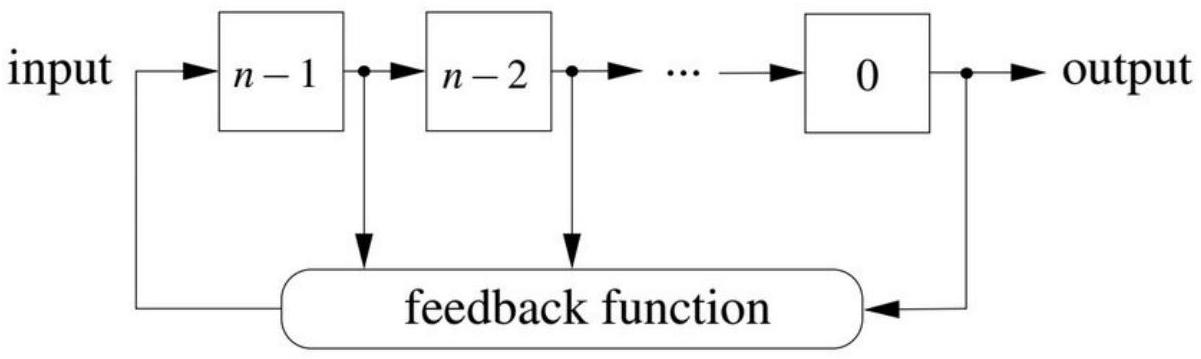
\includegraphics[max width=\columnwidth]{block_diagram.jpg}
  \caption{An $n$-bit FSR general structure.}
  \label{fig:block_diagram}
\end{figure}

\section{Results}
Preliminary results confirm the feasibility of our approach. Figure~\ref{fig:keystreams} shows 31 non-zero keystream plots produced by a 5-bit Fibonacci NLFSR with taps $[0,2,4,(2,3)]$. Each keystream exhibits unique local patterns, which our CNN leverages for classification.

\begin{figure}[ht]
  \centering
  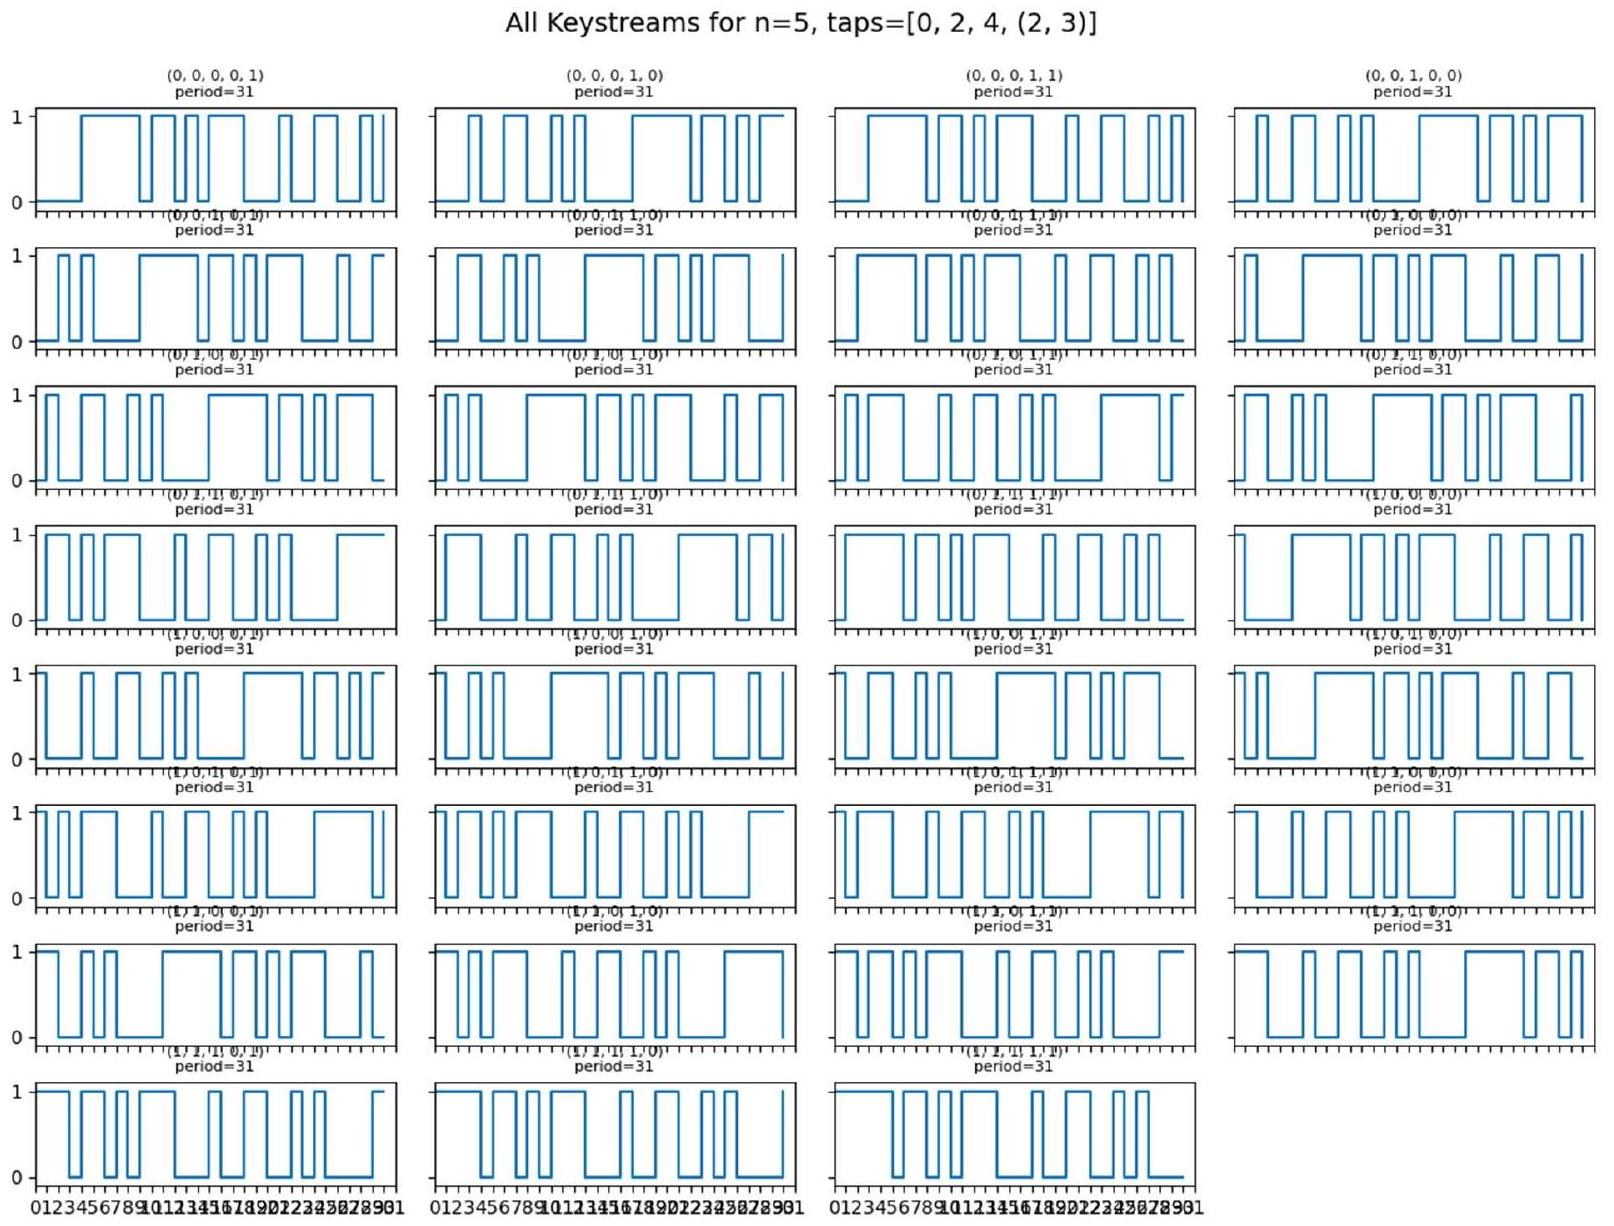
\includegraphics[max width=\columnwidth]{keystreams.jpg}
  \caption{31 Non-zero keystream plots for a 5-bit Fibonacci NLFSR.}
  \label{fig:keystreams}
\end{figure}

\section{Discussion}
Our approach demonstrates that each maximal-period feedback polynomial produces a unique "fingerprint" in its keystream. This insight advances NLFSR theory and provides a practical tool for cryptographic analysis. Challenges include scaling to larger $n$ and addressing class imbalance in the dataset.

\section{Conclusion}
This paper presents a novel ML-based pipeline for NLFSR analysis, combining exhaustive dataset generation, image encoding, and CNN classification. Future work will focus on scaling the methodology and exploring its applicability to other cryptographic primitives.

\section*{Acknowledgment}
The authors thank King Fahd University of Petroleum and Minerals for supporting this research.

\bibliographystyle{IEEEtran}
\bibliography{references}

\end{document}
